\subsection{IntAct curated physical interactions: do gated antigens co-complex?}
\label{sec:intact}
A biclonal AND gate assumes the two gated antigens can be engaged as
independent surface targets; if two antigens instead reside in a shared
membrane complex, cis-engagement could alter avidity, sterically couple the
two scFv binding events, or expose a single point of escape through loss of
the complex. We audited curated physical interactions from IntAct (EBI
PSICQUIC REST, MITAB 2.5) for all 205 genes in the study universe
(205 with a UniProt accession; the four pseudogene/unresolved cases carry
no record). For each gene we collected the PSICQUIC interaction count and
the full paginated MITAB record; evidence was restricted to human--human
pairs (taxid 9606 both sides) with a physical PSI-MI interaction type
(direct interaction, association, physical association, proximity), and
self-interactions were excluded from pairwise analysis.

\paragraph{Calibration gate.} Pre-registered gates PASSED: (G1) the ERBB2
partner set contains both canonical heterodimer partners EGFR and ERBB3
(observed present); (G2) for all 15 focus genes (7 antigens, 4 references,
4 intracellular controls) the paginated MITAB row count equals the
independent PSICQUIC count endpoint (observed 15/15); (G3) all 4
intracellular controls return nonzero curated counts, confirming the
pipeline resolves non-surface proteins (observed 4/4).

\paragraph{Antigen-pair co-complex test.} 0 of the 21 AND-gate
antigen pairs carry a curated human physical edge (none; fraction
0.000). A permutation null over 20{,}000 random 7-gene background
subsets gives $p=1.0$; a degree-matched null matching each antigen to a
background gene within $\pm25\%$ curated degree (20{,}000 valid draws)
gives $p=1.0$. No AND-gate antigen pair has a curated physical interaction: the gate's two arms are independent surface targets in the curated record, with no cis-complex to couple or short-circuit the two scFv engagements. Absence here is bounded by the study-bias audit below: low-degree antigens are simply under-probed.

\paragraph{Interaction degree: study-bias audit.} Median curated degree is
51 (gated) versus 15 (background) (Mann--Whitney $p=2e-06$);
any-record coverage is 96/99 gated versus 73/98 background (Fisher odds
ratio 10.959, $p=3e-06$). Stratified by epitope topology class, the
degree contrast is significant in multi-pass, unannotated (single-pass $p=0.086$, multi-pass $p=0.0003$, GPI $p=0.7758$, unannotated $p=0.0387$). Gated and background genes differ in curated interaction degree, so the interaction record is study-biased across the design split; pairwise conclusions must be read against the degree-matched null, which controls this bias.

\paragraph{Per-antigen interaction context.} \textbf{CA9} (curated degree 15); \textbf{CA12} (curated degree 12); \textbf{CLDN18} (curated degree 109); \textbf{CLDN6} (curated degree 20); \textbf{MSLN} (curated degree 27); \textbf{PSCA} (curated degree 103); \textbf{SLC39A6} (curated degree 50).

\begin{figure}[t]
\centering
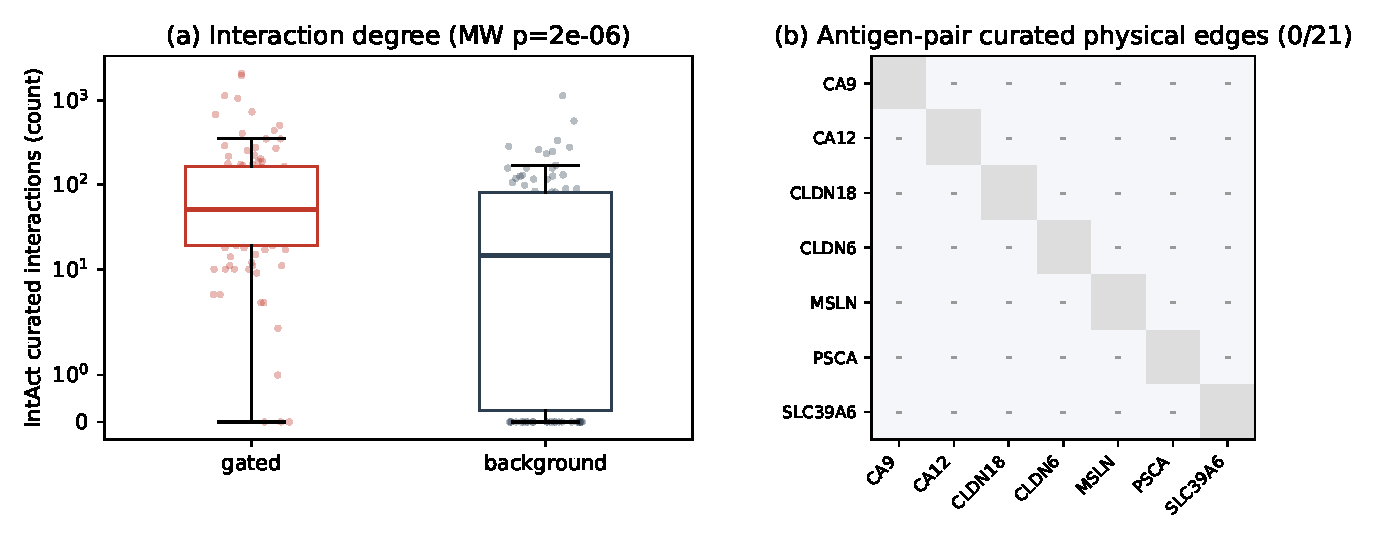
\includegraphics[width=\linewidth]{intact_fig.pdf}
\caption{IntAct curated interaction context. (a) Curated physical
interaction degree for gated versus background genes (symlog axis; boxes
show median and quartiles). (b) Pairwise curated physical edges among the
seven AND-gate antigens (Y = human physical curated edge in IntAct; grey
diagonal excluded).}
\label{fig:intact}
\end{figure}
